%!TEX root = report.tex
\chapter{Evaluation}

\section{Compare predictions to real data}
We can compare the predictions generated to the live bus arrivals data stored in the arrivals table. We can calculate the standard deviation of the difference in the predicted time and actual arrival time. This value will be the direct indicator of the accuracy of the predictions.

\section{Accuracy}
How accurate are the predictions?


\section{Performance}
\subsection{Tool}
\par We used \textit{siege}\cite{siege} to conduct the load test of our API endpoints. Our aim was to test the number requests the server could handle reliably at one time, and the response time it took.

\par \textit{Siege} takes in the number of users, the delay time between each page load, the test running time, and the list of URLs to send requests to as parameters. It then simulates the user behaviours to fire requests to the list of given URLs. At the end of the test, \textit{Siege} generates a report for the test, including metrics such as the transaction rate, and the response time of the target URLs.

\subsection{Preparation}
\par We generated a list of API URLs with random parameters for testing. We then ran the siege tests by fixing the test running time to be 1 minute, with 1 second of delay between each page load.

\subsection{Results}
\par We found out that currently, the server could reliably handle about 150 users to send requests concurrently, with an average response time of 15.78 seconds. Figure \ref{fig:performance} shows the results of our tests.

\begin{figure}
\centering
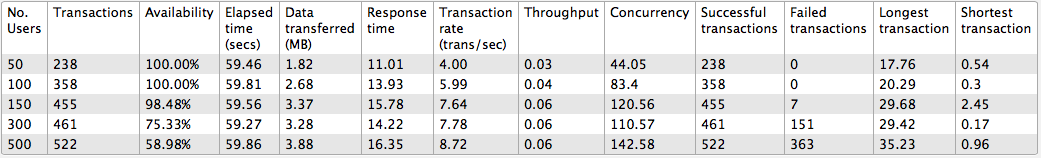
\includegraphics[width=\textwidth]{figures/performance.png}
\caption{\label{fig:performance} Result of Performance Test with Siege}
\end{figure}

\todo[inline]{plot graph from results}

\section{User feedback on UI}
We
How effective is it at warning delay?

